\documentclass[a4paper, 11pt]{article}

\usepackage{fullpage}

\usepackage[english,russian]{babel}
\usepackage[utf8]{inputenc}
\usepackage{amsmath, amsfonts, amssymb}
\usepackage{mathtools}
\usepackage{bm}

\usepackage{hyperref}
\usepackage{booktabs}
\usepackage{graphicx}
\usepackage{subcaption}

\usepackage[linesnumbered,ruled,vlined]{algorithm2e}
\SetKwInput{KwInput}{input}
\SetAlFnt{\small}

\usepackage{float}

\begin{document}

\begin{titlepage}
	\newpage
	
	\begin{center}
	%	Московский Государственный Университет им. М. В. Ломоносова \\
	\end{center}
	
	\vspace{8em}
	
	\begin{center}
		%\Large Кафедра Вычислительных Технологий и Моделирования \\ 
	\end{center}
	
	\vspace{2em}
	
	\begin{center}
		\textsc{\textbf{Введение в работу с неструктурированными сетками с помощью платформы INMOST и других инструментов}}
	\end{center}
	
	\vspace{6em}
	
	
	
	\newbox{\lbox}
	\savebox{\lbox}{\hbox{}}
	\newlength{\maxl}
	\setlength{\maxl}{\wd\lbox}
	\hfill\parbox{11cm}{
		%\hspace*{5cm}\hspace*{-5cm}Студент:\hfill\hbox {Иванов И. И.\hfill}\\
		%\hspace*{5cm}\hspace*{-5cm}Преподаватель:\hfill\hbox {Ануприенко Д. В.\hfill}\\
	%	\\
		%\hspace*{5cm}\hspace*{-5cm}Группа:\hfill\hbox {403}\\
	}
	
	
	\vspace{\fill}
	
	\begin{center}
		Москва \\ 2022
	\end{center}
	
\end{titlepage}

\setcounter{MaxMatrixCols}{20}


\section{Установка INMOST}

INMOST (\texttt{www.inmost.org, https://github.com/INMOST-DEV/INMOST}) -- разрабатываемая в ИВМ платформа, предоставляющая необходимые инструменты и структуры данных для решения различных уравнений на неструктурированных сетках. Язык разработки -- C++. Основной функционал, используемый в данном курсе -- работа с неструктурированными сетками и решение линейных систем. Остальные возможности INMOST, такие как автоматическое дифференцирование для построения матриц Якоби и распараллеливание на основе MPI, остаются за рамками данного курса.

Перед скачиванием рекомендуется завести некоторую начальную директорию, в которой затем будут располагаться INMOST и связанные с ним проекты. Перейдя в эту директорию, можно скачать INMOST следующей командой:
~\\

\texttt{git clone https://github.com/INMOST-DEV/INMOST.git}
~\\

Затем надо перейти в новую директорию и создать папку со сборкой:
~\\

\texttt{cd INMOST}

\texttt{mkdir build}

\texttt{cd build}
~\\

Для сборки используется CMake. Запускаем сборку:
~\\

\texttt{cmake ..}

\texttt{make}

\section{Установка пакета работы с сетками INMOST-GridTools}
Пакет INMOST-GridTools используется, чтобы научиться собирать проекты, зависящие от INMOST. Этот пакет содержит некоторые полезные утилиты для работы с сетками, а также ряд генераторов неструктурированных сеток в единичном кубе. По большей части, эти генераторы создают сетки с разными кривыми ячейками, которые создают проблемы для методов дискретизации, и эти сетки используются для проверки их работы. Генераторы сохраняют сетки в разных форматах, среди которых мы будем использовать формат VTK (Visualisation ToolKit) -- \texttt{.vtk}.

Установите INMOST-GridTools аналогично INMOST, \\адрес проекта -- \texttt{https://github.com/INMOST-DEV/INMOST-GridTools}.

\section{Установка ParaView}
ParaView (\texttt{https://www.paraview.org/}) -- повсеместно используемое средство визуализации, способное работать с файлами в формате VTK. Мы воспользуемся лишь малой частью возможностей ParaView. Необходимо скачать с официального сайта.

\section{Генерация сеток и их визуализация в ParaView}.
Научимся просматривать сетки в ParaView. Для этого в папке \texttt{build} проекта INMOST-GridTools запустите один из следующих исполняемых файлов:
\begin{itemize}
	\item Азамат -- \texttt{kershaw\_mesh}
	\item Антон -- \texttt{acute\_mesh}
	\item Ирина -- \texttt{sinusoidal\_mesh}
	\item Лев -- \texttt{hex\_mesh}
	\item Михаил -- \texttt{shestakov\_mesh}
	\item Софья -- \texttt{nonconvex\_mesh}
\end{itemize}
Как правило, нужно подать 2 аргумента -- число ячеек по горизонтальным осям и число ячеек по вертикальной оси.

Откройте \texttt{grid.vtk} в ParaView. Нажмите на зеленую кнопку \texttt{Apply}. Обший интерфейс представлен на рисунке \ref{fig:pv_gui}. Основная работа с данными на сетками в ParaView делается с помощью \textit{фильтров}. Среди \texttt{Filters} найдите \texttt{Clip}, задайте нормаль $[1~1~1]$ и отметьте галочку \texttt{Crinkle clip}, чтобы ячейки не резались. Примерный результат для одной из сеток представлен на рисунке \ref{fig:pv_gui}. Использует формат отображения сетки \texttt{Surface with edges}, чтобы видеть отдельные ячейки. В данный момент на сетке (в большинстве случаев) нет никаких данных, так что раскрасить сетку можно только в \texttt{Solid Color}.

\begin{figure}[h] \centering
		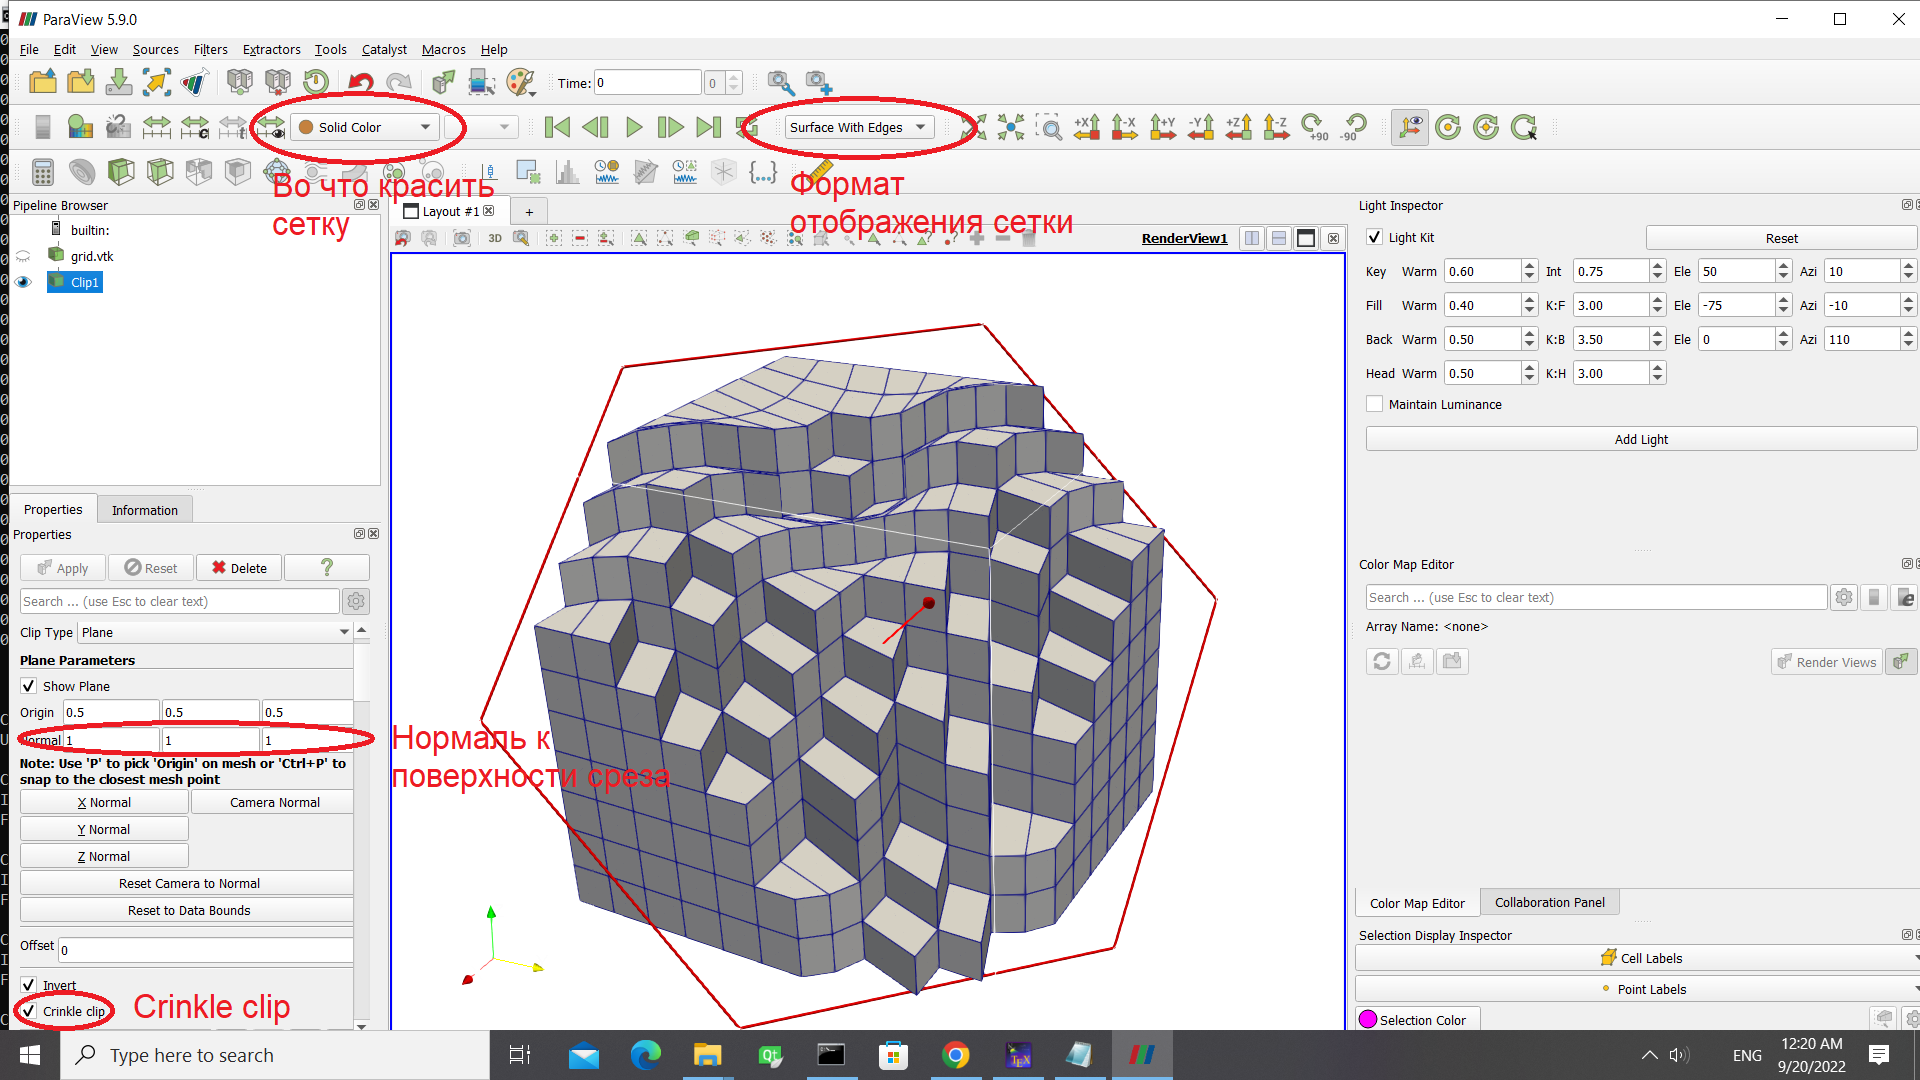
\includegraphics[scale=0.4]{pv_gui.png}
	\caption{Интерфейс ParaView\label{fig:pv_gui}}
\end{figure}

\section{Работа с данными на сетках в INMOST}

\subsection{Создайте свой проект}
Создайте директорию для своего проекта рядом с директориями \texttt{INMOST}, \texttt{INMOST-GridTools}. Поместите туда приложенные \texttt{CMakeLists.txt}, \texttt{main.cpp}. Создайте папку \texttt{build} и проверьте, что сборка идет успешно.

\subsection{Понятие тега}
Для записи данных на сетке в INMOST используется понятие \textit{тега} (ярлыка). При наличии объекта класса тег считается, что на некоторых сеточных элементах (узлах, ячейках, гранях) хранится информация, которую можно запросить для этих сеточных элементов. При создании тега указываются
\begin{itemize}
	\item имя тега,
	\item тип данных (как правило, целые или действительные числа),
	\item тип элементов, на которых определен тег, при этом для сразу нескольких типов запись имеет вид \texttt{CELL|FACE},
	\item тип элементов, где тег является разреженным, эта возможность нам не нужна, так что будет писать \texttt{NONE},
	\item размер тега: для скаляров это 1, для векторов -- 2 или 3; мы пока ограничимся скалярами.
\end{itemize} 

В приложенной программе на сетке создаются теги \texttt{Cell\_count} и \texttt{X\_Coord}. Первый тег определен на узлах и для каждого узла содержит число окружающих его ячеек. Второй тег определен на ячейках и содержит х-координату центроидов ячеек.

\subsection{Задания: вычисление норм ошибки, подсчет числа узлов в ячейках}
Даны сетки с тегами \texttt{U} и \texttt{U\_approx}, определенными в ячейках. Считается, что функции кусочно-постоянны на сетке. Найдите $C$- и $L_2$-нормы ошибки.

Создайте на ячейках тег и запишите для каждой ячейки число узлов.




\end{document}